\section{\CS: A Computational Fluid Dynamics code}
\label{sec:cs}
\CS is a computational fluid dynamics software designed to solve the
Navier-Stokes equations in the cases of 2D, 2D axisymmetric or 3D
flows. Development started in 1997, with a first release in 2000, and the
code has been released as free software under a GPL licence since 2007.
Its main module is designed for the simulation of flows which may be
steady or unsteady, laminar or turbulent, incompressible or potentially
dilatable, isothermal or not. Scalars and turbulent fluctuations of scalars can
be taken into account. The code includes specific modules, referred to as
``specific physical models'', for the treatment of atmospheric flows, Lagrangian particle
tracking, semi-transparent radiative transfer, gas combustion, pulverised coal
combustion, electricity effects (Joule effect and electric arcs) and
compressible flows. \CS relies on a finite volume discretisation and
allows the use of various mesh types which may be hybrid (containing several
kinds of elements) and may have structural non-conformities (hanging nodes). The
parallelization is based on standard spatial partitioning with ghost cells
that facilitate data passing between adjacent cells lying across the boundaries
of disconnected parts using the Message Passing Interface. More
technical details are presented in~\cite{cs2004} and ~\cite{userguide},
and many resources are available at \url{http://www.code-saturne.org}.
\CS is also used as a base for the NEPTUNE\_CFD code, specialized in
multiphase flows, and which uses a different time stepping scheme,
but mostly the same volume discretization scheme.

As \CS is used for industrial cases involving complex flows, with turbulence
modeling requiring sufficiently fine resolution, large meshes are often
needed. In 2000, the largest meshes used for actual studies were around
1.5 million cells; today, they have reached up to 350 million cells.
More common studies use meshes about 10 times smaller than that.
Meshes up to 3.2 billion cells have been tested for a few time steps, to
ensure the code's internal mechanisms work well at scale.

\CS focuses on the solver, and its uses requires external tools for the
major part of the meshing and visualisation tasks, though the code itself offers
major preprocessing features to make these easier, such as parallel joining
of independently-built and read submeshes (whether conforming or not),
and user-definable postprocessing functions. Many input mesh and visualisation
output formats are supported (including the EDF and CEA MED format,
and the standardized CGNS format).

~\
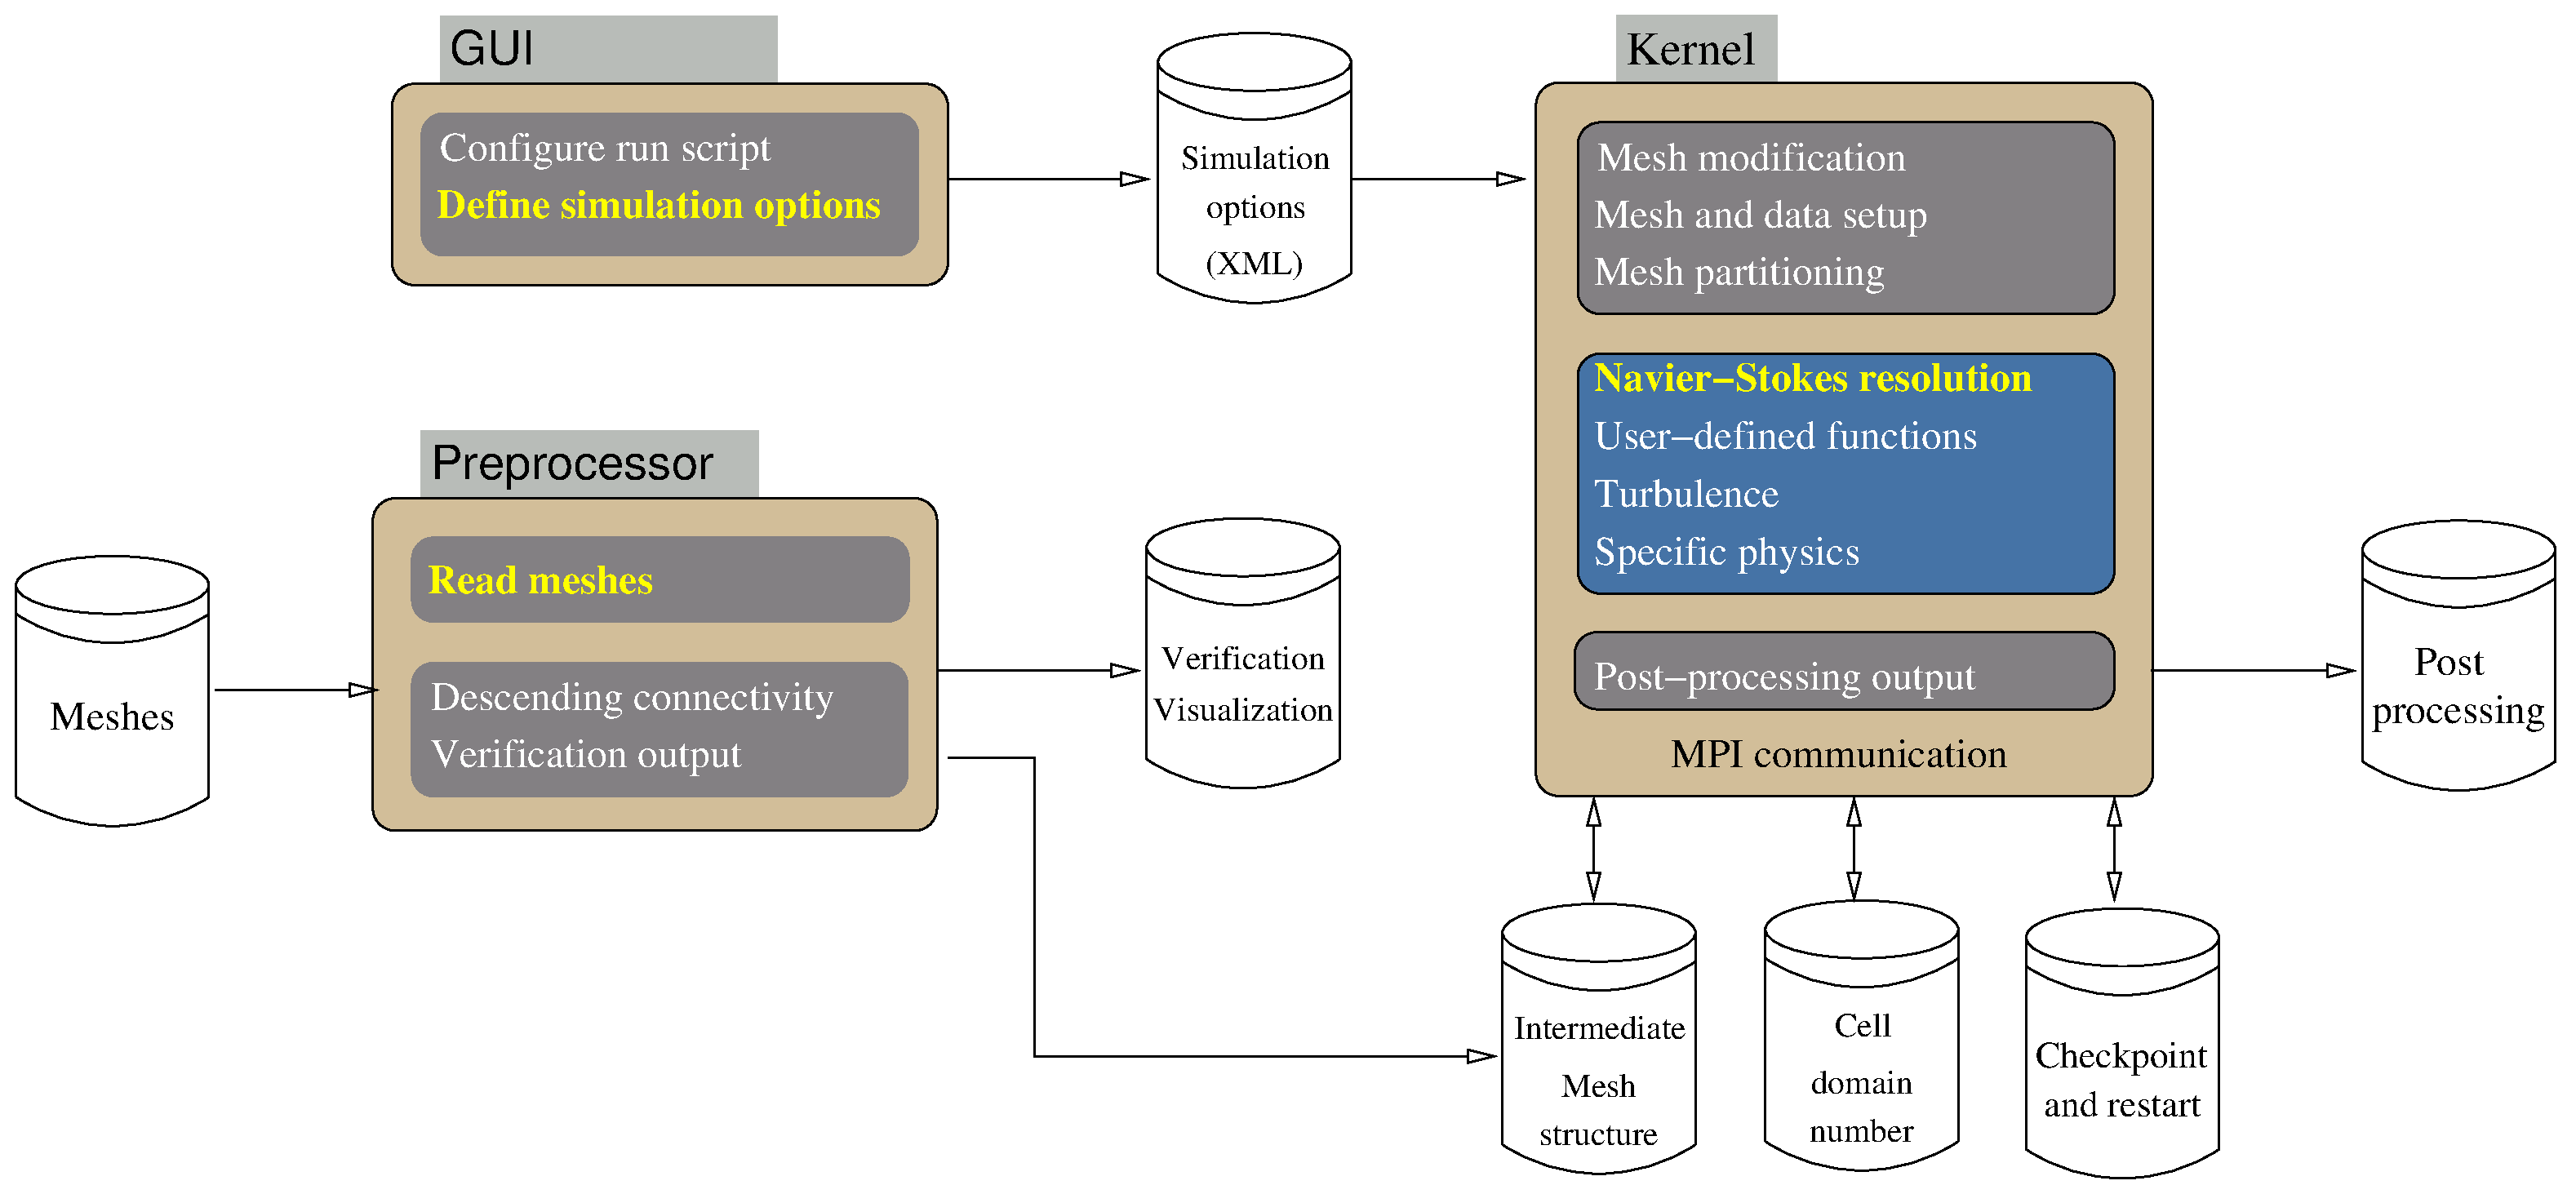
\includegraphics[scale=0.2]{pictures/cs_components.eps}
\captionof{figure}{\CS toolchain components.}
\label{fig:cs_components}
\vspace{+0.04in}
~\

The number of separate executable tools is quite reduced, with a few
interactive tools and associated commands designed for data setup.

To make the use of HPC as seamless as possible, without multiplying the
number of tools or requiring complex libraries or dependencies,
mesh, checkpoint/restart, and postprocessing output files
are partitioned independently: in addition to the connectivity of each
local mesh, which is described with a local numbering, global ids are also
maintained, for import and export purposes, and for ghost cell to
local cell matching. Multiple ranks participate in reading and writing
files using MPI-IO.

Typically, computational resource requirements are primarily determined
either by the time to solution, or the size of the model. For time to
solution, the number of cores may be selected in order to solve the problem
in a given time. In practice, optimal performance is often obtained
in a range of 30~000 to 60~000 cells per rank on a typical HPC cluster
(this being the best compromise between communication latency and
cache behavior). On machines with very good network/compute performance
ratios, such as IBM Blue Genes or Cray X series, this range may be
a bit wider.
